\chapter{Linear Algebra} \label{ch:linear algebra}
        \section{Introduction}
        \begin{itemize}
            \item problems in various fields of science and mathematics involve the solution of sets of linear equations.
            Suppose you have solved two simultaneous linear equations and have found $x=2$ and $y=-3$. We can think of
            $x=2$, $y=-3$ as the point $(2,-3)$ in the $(x,y)$ plane. Since two linear equations represent two straight lines,
            the \emph{solution} is then the \textit{point} of intersection of the lines.

            \item The language of vectors is very useful in studying sets of simultaneous equations. 
            \textit{Quantities} such as the velocity of an object, which have both \emph{magnitude} and \emph{direction}. 
            Such quantities are called \textbf{vectors}; contrast them with such quantities as mass,
            which have \textit{magnitude} only and are called \textbf{scalars}.
            \item Vector formulas are independent of the choice of coordinate system.
            \item A vector equation in two dimensions is equivalent to two component equations.
        \end{itemize}

        \section{Matrices: Row Reduction}
            \begin{itemize}
                \item A matrix (plural: matrices) is just a rectangular array of quantities, such as
                \begin{align} \label{matrix example}
                    A= \begin{bmatrix} 
                        1 & 5 & -2 \\
                        -3 & 0 & 6 
                    \end{bmatrix}
                \end{align}
                \item The $A$ letter does not have a numerical value; it simply stands for the array.
                \item To indicate a number in the array, we will write $A_{ij}$ where $i$ is the 
                \textit{row} number and $j$ is the \textit{column} number.
                \item We will call a matrix with $m$ rows and $n$ columns as \textit{$m$ by $n$ matrix}.
                \item \textbf{Transpose of a Matrix} We write:
                \begin{align} \label{transpose example}
                    A= \begin{bmatrix} 
                    1 & -3 \\ 
                    5 & 0 \\
                    -2 & 6
                    \end{bmatrix}
                \end{align}
                and call $A^T$ the transpose of the matrix A in Matrix\eqref{matrix example}.
                \item To transpose a matrix, we simply write the rows as columns.
                \item Not that, $(A^T)_{ij} = A_{ji}$
                \item Consider the set of equations of:
                \begin{align}\label{set of equations}
                    \begin{cases}
                        2x - z =2\\
                        6x + 5y + 3z = 7\\
                        2x - y = 4
                    \end{cases}
                \end{align}
                \item Let's agree in organizing them in \textit{standard form}, each column be for a specific variable.
                \item There are three markable matricies to extract from \eqref{set of equations}; 
                first one is the \textit{matrix of the coefficients}
                \begin{align} \label{matrix of the coefficiants}
                    M= \begin{bmatrix}
                        2 & 0 & -1 \\
                        6 & 5 & 3 \\
                        2 & -1 & 0
                    \end{bmatrix}
                \end{align}
                Also, there are $3\times1$ matrices, $r$ and $k$.
                \begin{align}
                    r= \begin{bmatrix}
                        x \\ y \\ z
                    \end{bmatrix}, \quad
                    k= \begin{bmatrix}
                        2 \\ 7 \\ 4
                    \end{bmatrix}
                \end{align}
                \item The Eqs\eqref{set of equations} can be written in matrix as $Mr=k$.
                \item Now we want to write Eqs\eqref{set of equations} in an \textit{augmented matrix}
                \begin{align} \label{augmented matrix}
                    A= \begin{bmatrix}
                        2 & 0 & -1 & 2 \\
                        6 & 5 & 3 & 7 \\
                        2 & -1 & 0 & 4
                    \end{bmatrix}
                \end{align}
                and then solve it by the \textit{row reduction} with the following \textit{elementary row operations}:
                \begin{align}  \label{elementry row operations}
                    \coloredpar{
                    \begin{enumerate}
                        \item Interchange two rows.
                        \item Multiply (or divide) a row by a (nonzero) constant.
                        \item Add a multiple of one row to another; this includes 
                        subtracting, that is, using a negative multiple.
                    \end{enumerate}}
                \end{align}
                \item If the last row in a rediced augmented matrix is like $0 \times z=5$, which cannot be 
                true for any finite number on $z$, then it is called \textit{inconsistent}.
                \item \textbf{Rank of a Matrix} The number of nonzero rows remaining when a matrix has been 
                row reduced is called the rank of the matrix.
                \begin{align}
                    \coloredpar{
                        \begin{enumerate}
                            \item If $(\rank M)<(\rank A)$, the equations are inconsistent and there is no solution.
                            \item If $(\rank M)=(\rank A)=n$(\# of unknowns), there is one solution.
                            \item If $(\rank M)=(\rank A)=R<n$, then $R$ unknowns can be found in terms of the remaining $n-R$ unknowns.
                        \end{enumerate}}
                \end{align}
            \end{itemize}

        \section{Determinants; Carmer's Rule}
            For a square matrix, however, there is a useful number called the determinant of the matrix.
            \begin{itemize}
                \item For a $2\times2$ Matrix:
                \begin{align} \label{det of 2by2 matrix}
                    A= \begin{bmatrix}
                        a & b \\
                        c & d
                    \end{bmatrix}, \quad
                    det\, A = \begin{vmatrix}
                        a & b \\
                        c & d
                    \end{vmatrix} =ad-bc
                \end{align}
                \item If we remove one row and one column from a determinant of order $n$, 
                    we have a determinant of order $n-1$.
                \item When removing the \textit{row} and \textit{column} containing the element $a_{ij}$ and call the 
                    remaining determinant $M_{ij}$, which is called the \textbf{minor} of $a_{ij}$.
                \item The \textbf{cofactor} of $a_{ij}$ is: \coloredeq{eq:cofactor of a_ij}{C_{ij}=(-1)^{i+j}M_{ij}}
                \item In general, for $n \times n$ matrix we have,
                \begin{align}
                    \label{eq:general det of nXn matrix}
                    \det{A} = \sum_{j=1}^n\, a_{ij}C_{ij}, \quad \text{where $j$ is fixed}
                \end{align}
                \item The signs goes like $\begin{vmatrix}
                    + & - &  \\
                    - & + &  \\
                    &   &  \ddots
                \end{vmatrix}$.
            \end{itemize}

            \paragraph{$\bigstar$} The value of a \textit{determinant}: Multiply each element of one row (or one column) 
                by its cofactor and add the results.
            
            \textbf{Useful Fact About Determinants}:
            \begin{align}
                \coloredpar{\begin{enumerate}
                    \item If each element of one row (or one column) of a determinant is multiplied by a number $k$, 
                    the value of the determinant is multiplied by $k$.
                    \item The value of a determinant is zero if
                    \begin{enumerate}
                        \item all elements of one row (or column) are zero; or if
                        \item two rows (or two columns) are identical; or if
                        \item two rows (or two columns) are proportional.
                    \end{enumerate}
                    \item If two rows (or two columns) of a determinant are interchanged, 
                    the value of the determinant changes sign.
                    \item The value of a determinant is unchanged if
                    \begin{enumerate}
                        \item rows are written as columns and columns as rows; or if
                        \item we add to each element of one row, $k$ times the corresponding element of another row, 
                        where k is any number (and a similar statement for columns).
                    \end{enumerate}
                \end{enumerate}}
            \end{align}

            \paragraph{Carmer's Rule} This is a formula in terms of determinants for the solution of $n$ linear equations 
            in $n$ unknowns when there is exactly one solution.\\
            Let's start with the following equations:
            \begin{align} \label{eq:equations set example}
                \begin{cases}
                    a_1x + b_1y = c_1 \\
                    a_2x + b_2y = c_2
                \end{cases}
            \end{align}
            If we multiply the first equation by $b_2$, the second by $b_1$, and then subtract the
            results and solve for x, we get if $(a_1b_2 - a_2b_1 \neq 0)$
            \begin{align} \label{eq:equations set example:1}
                x = \frac{c_1b_2 - c_2b_1}{a_1b_2 - a_2b_1}, \quad 
                y = \frac{a_1c_2 - a_2c_1}{a_1b_2 - a_2b_1}
            \end{align}
            Using the definition \eqref{det of 2by2 matrix} we can write Eq.\eqref{eq:equations set example:1}
            \begin{align}
                x = 
                \frac{\begin{vmatrix}
                    c_1 & b_1 \\
                    c_2 & b_2
                \end{vmatrix}}
                {\begin{vmatrix}
                    a_1 & b_1 \\
                    a_2 & b_2
                \end{vmatrix}} = \frac{1}{D}
                \begin{vmatrix}
                    c_1 & b_1 \\
                    c_2 & b_2
                \end{vmatrix}, \quad\quad
                y = 
                \frac{\begin{vmatrix}
                    a_1 & c_1 \\
                    a_2 & c_2
                \end{vmatrix}}
                {\begin{vmatrix}
                    a_1 & b_1 \\
                    a_2 & b_2
                \end{vmatrix}} = \frac{1}{D}
                \begin{vmatrix}
                    a_1 & c_1 \\
                    a_2 & c_2
                \end{vmatrix}, \quad D \neq 0
            \end{align}
            \paragraph{$\bigstar$} To remember it, the denominator for both $x$ and $y$ is the 
            \textit{determinant of the coefficients},for the numerator for $x$ replace its column with 
            the $k$ matrix (constants column), and do so for $y$.

            \begin{align} \label{Carmer's Rule for solving n eqs}
                \coloredpar{
                    This method of solution of a set of linear equations is called Cramer’s rule. 
                    It may be used to solve $n$ equations in $n$ unknowns if $D \neq 0$; the solution then consists of 
                    one value for each unknown. The denominator determinant D is the $n$ by $n$ determinant of the 
                    \textit{coefficients} when the equations are arranged in standard form. The numerator determinant for 
                    each unknown is the determinant obtained by replacing the column of coefficients of that 
                    unknown in D by the constant terms from the right-hand sides of the equations. Then to find 
                    the unknowns, we must evaluate each of the determinants and divide.}
            \end{align}
            
            \paragraph{Rank of Matrix} Here is another way to find the rank of a matrix.
            A submatrix means a matrix remaining if we remove some rows and/or remove some 
            columns from the original matrix. To find the rank of a matrix, we look at all 
            the square submatrices and find their determinants. The \textit{order of the largest
            nonzero determinant} is the rank of the matrix.

        \section{Vectors}
            \paragraph{}{Notation} We shall indicate a vector by a boldface letter (for example, \textbf{A}) and a 
            component of a vector by a subscript (for example $A_x$ is the $4$ component of \textbf{A}). 
            For handwriting you should write a vector with an arrow (like, $\vec{A}$).

            \paragraph{Magnitude of a Vector} The \textit{length} of the arrow representing a vector $\textbf{A}$
            is called the \textit{length} or the \textit{magnitude} of \textbf{A} (written $|\textbf{A}|$ or $A$) or
            the \textit{norm} of \textbf{A} (written $||\textbf{A}||$). Note the use of A to mean the magnitude of \textbf{A}.

            \paragraph{$\bullet$} By the Pythagorean theorem, we find
            \coloredeq{eq:Pythagorean for vectors}{A = |\vec{A}| = \sqrt{A_x^2 + A_y^2 + A_z^2}}

            \paragraph{Addition of Vectors} There two ways to add vectors: 
            Addition of Vectors
            by the parallelogram law: To find $\vec{A} + \vec{B}$, place the tail of 
            $\vec{B}$ at the head of $\vec{A}$ and draw the vector from the tail of $\vec{A}$ to the head of $\vec{B}$.
            Or by adding their components togather, like $A_x + B_x$ and $A_y + B_y$. They follow:
            \begin{align} \label{vectors properties}
                \vec{A} + \vec{B} = \vec{B} + \vec{A}, \quad \text{(commutative law for addition)};\\
                (\vec{A} + \vec{B}) + \vec{C} = \vec{A} + (\vec{B} + \vec{C}), \quad \text{(associative law for addition)}.
            \end{align}
            \paragraph{$\bullet$} In other words, vectors may be added together by the usual laws of algebra.
            They can be multiplied by a number. Ane we can define vectors substraction so:
            $$ \vec{A} - \vec{B} = \vec{A} + (-\vec{B}) $$

            \paragraph{$\bullet$} The \textbf{zero vector} is a vector of zero magnitude; its 
            components are all zero and it does not have a direction.\\
            A vector of length or magnitude 1 is called a \textbf{unit vector}. 
            Then for any $\vec{A} \neq 0$, the vector $\vec{A}/|\vec{A}|$ is a unit vector.

            \begin{wrapfigure}{r}{0.2\linewidth}
                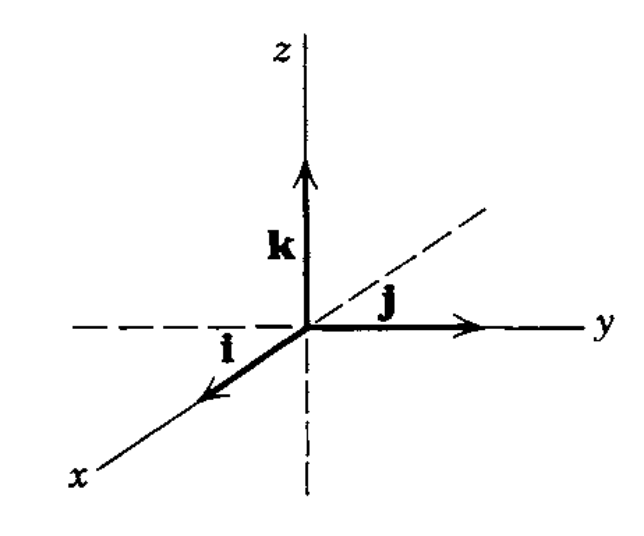
\includegraphics[width=0.9\linewidth]{figures/basis vectors.png}
                \caption{The unit basis vectors in a rectangular system.}
                \label{fig:basis vectors}
            \end{wrapfigure}

            \paragraph{Vectors in Terms of Components} We consider a set of rectangular axes as in Fig.\eqref{fig:basis vectors}
            let $\ihat $ be a unit vector in the positive $x$ direction; $\jhat $ and $\khat $
            in $y$ and $z$ positive direction. For $\vec{A}$
            \begin{align}
                \vec{A} = A_x\ihat  + A_y\jhat  + A_z\khat 
            \end{align} 
            The vectors $\ihat , \jhat , \khat $ are called \textit{unit basis vectors}.

            \paragraph{Multiplication of Vectors} There are two kinds of product of two vectors. 
            One, called the \text{scalar} product (or \textbf{dot product} or \textbf{inner product}), 
            gives a result which is a scalar; the other, called the \textit{vector product} 
            (or \textbf{cross product}), gives a vector answer.

            \paragraph{Scalar Product} For vectors $\vec{A}$, and $\vec{B}$, and the angle $\theta$($\le 180^\circ$) between them,
            we have:
            $$ \vec{A} \cdot \vec{B} = (\ihat A_x +\jhat A_y +\khat A_z) \cdot (\ihat B_x +\jhat B_y +\khat B_z) $$
            \coloredeq{eq:dot product}{\vec{A} \cdot \vec{B} = |\vec{A}||\vec{B}|\cos{\theta} = A_xB_x + A_yB_y + A_zB_z}
            The dot product in Eq.\eqref{eq:dot product} holds the commutative law.\\
            And the distributive law.

            \paragraph{$\bullet$} A vector dot itself gives its magnitude:
            $$ \vec{A} \cdot \vec{A} = |\vec{A}|^2\cos{0} = |A|^2 = A^2 $$

            \paragraph{Perpendicular and Parallel Vectors}  % (fold)
            \label{par:Perpendicular and Parallel Vectors}
            If two vectors are perpendicular, then $\cos{\theta} = 0$; thus
            \coloredeq{eq:Perp. vectors with dot product}{
                \begin{aligned}
                    \vec{A} \cdot \vec{B} &= A_xB_x + A_yB_y + A_zB_z = 0, && \text{if $\vec{A}$ and $\vec{B}$
                    are perpendicular vectors.} \\
                    \frac{A_x}{B_x} &= \frac{A_y}{B_y} = \frac{A_z}{B_z}, && 
                    \text{if $\vec{A}$ and $\vec{B}$ are perpendicular vectors.}
                \end{aligned}
            }
            % paragraph Perpendicular and Parallel Vectors (end)
            \paragraph{Vector Product} % (fold)
            \label{par:Vector Product}
            The vector or cross product of $\vec{A}$ and $\vec{B}$ is written $\vec{A} \times \vec{B}$. By
            definition, $\vec{A} \times \vec{B}$ is a vector whose magnitude and direction are given as follows:
            
            \begin{align} \label{eq:cross product magintude}\coloredpar{
                $$ |\vec{A} \times \vec{B}| = |\vec{A}||\vec{B}|\sin{\theta}, $$
                The direction of $\vec{A} \times \vec{B}$ is perpendicular to the 
                plane of $\vec{A}$ and $\vec{B}$, using \textit{right-hand rule}}
            \end{align}
            
            \paragraph{Intresting properties:}
            \coloredeq{eq:cross product properties}
            {\begin{aligned}
                \vec{A} \times \vec{B} &= - \vec{B} \times \vec{A}  && \text{not commutative,}\\
                \vec{A} \times \vec{B} &= 0 \quad && \parbox[c]{0.4\linewidth}{if $\vec{A}$ and $\vec{B}$ are parallel or antiparallel,}\\
                \vec{A} \times \vec{A} &= 0 \quad && \text{for any $\vec{A}$}
            \end{aligned}}
            % paragraph Vector Product (end)
                  
            
            \paragraph{$\bigstar$} A good way to remember the basis-unit vectors cross-product is 
            to write them cyclically. Reading around the circle counterclockwise (positive $\theta$ direction), 
            we get the positive products (for example, $\ihat  \times \jhat  = \khat $); reading 
            the other way we get the negative products (for example, $\ihat  \times \khat  = -\jhat $). This works with 
            the \textit{right-haned systems}.

            To write A × B in component form we need the distributive law, namely
            \begin{align} \label{eq:cross product distributive law}
                \vec{A} \times (\vec{B} + \vec{C}) = \vec{A} \times \vec{B} + \vec{A} \times \vec{c}
            \end{align}
            Thus we have:
            \coloredeq{eq:cross product vector}{
                \begin{aligned}
                    \vec{A} \times \vec{B} &= 
                    (\ihat A_x +\jhat A_y +\khat A_z) \times (\ihat B_x +\jhat B_y +\khat B_z)\\
                    &=\ihat (A_yB_z - A_zB_y) + \jhat (A_zB_x - A_xB_z) + \khat (A_xB_y - A_yB_x)\\
                    &= \begin{vmatrix}
                        \ihat  & \jhat  & \khat  \\
                        A_x & A_y & A_z \\
                        B_x & B_y & B_z
                    \end{vmatrix}
                \end{aligned}
            }
                    
        \section{Lines and Planes}
            In analytic geometry a point is a set of three coordinates $(x,y,z)$; we shall think of 
            this point as the \textit{head} of a vector $\vec{r} = \ihat x + \jhat y + \khat z$ with 
            \textit{tail} at the \texttt{origin}.
            In two dimensions, we write the equation of a \textit{straight line} through $(x_0,y_0)$ with slope $m$ as
            \begin{equation}
                \label{eq:straight line}
                \frac{y-y_0}{x-x_0} = m
            \end{equation}

            \paragraph{$\bullet$} Suppose, instead of the slope, we are given a vector in the direction 
            of the line, say $\vec{A} = \ihat a+\jhat b$. Then the line through $(x_0,y_0)$ and parallel to
            $\vec{A}$ we can write its equation. If we have two points on the line from $(x_0,y_0)$
            to any point $(x,y)$, then the vector $\vec{r} - \vec{r_0}$ with components $x-x_0 $ and $y-y_0$:
            \begin{align}
                \label{eq:vector bewtween two points}
                \vec{r} - \vec{r_0} = (x-x_0)\ihat  + (y-y_0)\jhat 
            \end{align}
            Since this vector is parallel to $\vec{A}$, then their components are proportional, so (for $a, b\neq 0$):
            \begin{align}
                \label{eq:line equation:2}
                \frac{x-x_0}{a} = \frac{y-y_0}{b} && or\quad \frac{y-y_0}{x-x_0} = \frac{b}{a}
            \end{align}
            The equation is for a given \textbf{line}, see tht Eq.\eqref{eq:straight line} and 
            Eq.\eqref{eq:line equation:2} are identical.

            \paragraph{$\bullet$} Since $\vec{r} -\vec{r_0}$ and $\vec{A}$ are parallel, thus they are only differen 
            by a factor of $t$, so
            \begin{align}
                \label{eq:r and A equivlent}
                \vec{r} -\vec{r_0} = \vec{A} t \quad or \quad \vec{r} = \vec{r_0} + \vec{A} t
            \end{align}
            Then theier \textit{components form}:
            \begin{align}
                \begin{aligned}
                    x - x_0 = at \\
                    y - y_0 = bt
                \end{aligned} \quad or \quad
                \begin{aligned}
                    x = x_0 + at \\
                    y = y_0 + bt
                \end{aligned}
            \end{align}
            Eliminating $t$ yields the equation of the line in Eq.\eqref{eq:line equation:2}
            
            \paragraph{$\bullet$} In three dimensions, we want the equations of
            a straight line through a given point $(x_0,y_0,z_0)$ and parallel to a given vector 
            $\vec{A} = a\ihat  + b\jhat  + c\khat $. If $(x,y,z)$ is any point on the line, the 
            vector joining $(x_0,y_0,z_0)$ and 
            $(x,y,z$) is parallel to $\vec{A}$. Then,
            \coloredeq{eq:symmetric line in 3D}{
                \begin{aligned}
                    \frac{x-x_0}{a} &= \frac{y-y_0}{b} = \frac{z-z_0}{c} && \text{$a, b, c \neq 0$}\\
                    \frac{x-x_0}{a} &= \frac{y-y_0}{b} , z=z_0 && \text{if say $c=0$}
                \end{aligned} 
            }
            \begin{wrapfigure}{r}{0.2\linewidth}
                \label{fig:parametric line}
                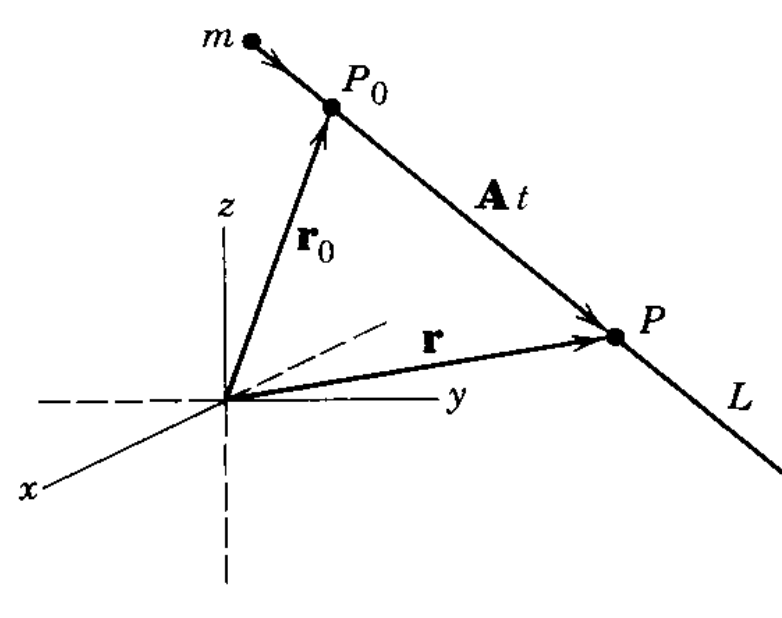
\includegraphics[width=0.9\linewidth]{figures/parametric line.png}
                \caption{}
            \end{wrapfigure}
            The paramtric equations for a line, see Fig.\eqref{fig:parametric line}, from Eq.\eqref{eq:symmetric line in 3D}
            \coloredeq{eq:paramtric equations}{
                \vec{r} = \vec{r_0} + \vec{A}t \quad or 
                \begin{aligned}
                    \begin{cases}
                        x = x_0 + at \\
                        y= y_0 + bt \\
                        z = z_0 +ct
                    \end{cases}
                \end{aligned} 
            }
    
            \paragraph{$\bullet$} Suppose we want the equation of a 
            straight line $L$ through the point $(x_0, y_0)$ and \texttt{perpendicular} to a given vector $\vec{N} = a\ihat +b\jhat $.
            Let the vector in Eq.\eqref{eq:vector bewtween two points} lies along the line but to be perpendicular
            to $\vec{N}$. \textit{Recall} from \eqref{eq:Perp. vectors with dot product}, we have 
            $(\vec{r}-\vec{r_0}) \cdot \vec{N} = 0$, thus their components
            \begin{align}
                \label{eq:Perp. line equation}
                a(x-x_0) + b(y-y_0) = 0 \quad or \quad \frac{y-y_0}{x-x_0} =- \frac{a}{b}
            \end{align}
            This is the equation for a line that is perpendicular to $\vec{N}$
    
            \paragraph{$\bullet$} In 3D, we can use this method to assign an equation for a plne. 
            Suppose that two points on the plane, $(x_0, _0, z_0)$ and $(x, y, z)$ is any point and represented by the
            vector in \eqref{eq:vector bewtween two points}.\\
            If $\vec{N} = a\ihat +b\jhat +c\khat $ is a normal vector to the plane, we have $(\vec{r}-\vec{r_0}) \cdot \vec{N} = 0$, so 
            \coloredeq{eq:3D plane equation}{
                \begin{aligned}
                    a(x - x_0) + b(y - y_0) + c(z - z_0) &= 0,\\
                    ax + by + cz &= d \quad \textit{where} \quad d=ax_0 + by_0 + cz_0
                \end{aligned}
            }

        \section{Matrix Operations}
            In Section 2 we used matrices simply as arrays of numbers. Now we want to go farther into the subject 
            and discuss the meaning and use of multiplying a matrix by a number and of combining matrices by addition, 
            subtraction, multiplication, and even (in a sense) division.
            
            \paragraph{Matrix Equations} % (fold)
            \label{par:Matrix Equations}
            Two matrices are only equal if they are identical, for example,
            \begin{align}
                \begin{bmatrix}
                    w & m \\
                    r & k
                \end{bmatrix} = 
                \begin{bmatrix}
                    4 & 5i \\
                    5 & 0
                \end{bmatrix}
            \end{align}
            then $w=4, \quad m=5i, \quad r=5, \quad k=0$.\\ Remeber this consept in the equation 
            $z = x + iy = 2 - 3i$ is equivalent to the two real equations $x = 2$, $y = -3$; \\
            a vector equation in three dimensions is equivalent to three component equations.
            % paragraph Matrix Equations (end)
            \paragraph{Multiplication of a Matrix by a Number} % (fold)
            \label{par:Multiplication of a Matrix by a Number}
            We can write a vector $\vec{A} = a\ihat  + b\jhat  + c\khat $ in matrix-like way,
            \begin{equation}
                \begin{aligned}
                \label{eq:vector in matrix}
                A = \begin{bmatrix}
                    a\\
                    b\\
                    c
                \end{bmatrix}\, \text{a column matrix or column vector,} \\
                A^T= \begin{bmatrix}
                    a & b & c
                \end{bmatrix}\, \text{called a row matrix or row vector.}
                \end{aligned}
            \end{equation}
            The row matrix $A^T$ is the transpose of the column matrix $A$
            % paragraph Multiplication of a Matrix by a Number (end)
            
            \paragraph{$\bullet$} Suppose we multiply the vector 
            $\vec{A}$ by a constant $C$, them $C\vec{A} = aC\ihat  + bC\jhat  + cC\khat $ and its matrix becomes
            \begin{align}
                A = \begin{bmatrix}
                    aC & bC & cC
                \end{bmatrix}
            \end{align}
            \paragraph{$\bigstar$}
            Thus when a matrix is multiplied by a number each element is multiplied by it.

            \coloredpar{Multiplying a matrix 
            by a number $k$ means multiplying every element by $k$,\\ But multiplying just one \textit{row} of a determinant
            by $k$ multiplies the determinant by $k$. Thus $\det{kA} = k^2 \det{A}$ for a 2 by 2 matrix.}
            \paragraph{Addition of Matrices} % (fold)
            \label{par:Addition of Matrices}
            When we add vectors algebraically, we add them by components. Matrices are added in the
            same way, but by adding \textit{corresponding elements}. If the two matrices have different $m$ by $n$,
            we say that the sum is undefined or meaningless.
            % paragraph Addition of Matrices (end)

            \paragraph{Multiplication of Matrices} % (fold)
            \label{par:Multiplication of Matrices}
            Let us start by defining the product of two matrices,
            \begin{align}
                \label{eq:multiply two 2X2 matrices}
                AB = \begin{bmatrix}
                    a & b \\
                    c & d
                \end{bmatrix}
                \begin{bmatrix}
                    e & f \\
                    g & h
                \end{bmatrix} =
                \begin{bmatrix}
                    ae+bg & af+bh\\
                    ce+dg & cf+dh
                \end{bmatrix} = C
            \end{align}
            Each row for each column. :“row times column”.
            \coloredeq{eq:matrix multiplication in indeces}{
                \parbox{0.6\linewidth}{The element in row $i$ and column $j$ of the product matrix $AB$ 
                is equal to row $i$ of $A$ times column $j$ of $B$. In index notation}
                 &&
                \begin{aligned}
                    (AB)_{ij} = \sum_k\, A_{ik}B_{kj}
                \end{aligned}
            }
            \coloredpar{The product $AB$ (in that order) can be found if and only if the number of elements 
            in a \textit{row} of $A$ equals the number of elements in a \textit{column} of $B$; the matrices $A$, $B$ in that 
            order are then called \textbf{conformable}. \\(Observe that the number of rows in \textit{A} and of columns 
            in $B$ have nothing to do with the question of whether we can find $AB$ or not.)}
            
            \coloredeq{eq:commutator}{[A,B]=AB-BA= \text{\textit{commutator} of $A$ and $B$.}}
            % paragraph Multiplication of Matrices (end)
            
            \paragraph{Zero Matrix} % (fold)
            \label{par:Zero Matrix}
            The \textbf{zero} or \textbf{null} matrix means one with all its elements equal to zero. 
            It is often abbreviated by 0, but we must be careful about this
            % paragraph Zero Matrix (end)

            \paragraph{Identity Matrix or Unit Matrix} % (fold)
            \label{par:Identity Matrix or Unit Matrix}
            This is a square matrix with every element of the main diagonal
            equal to 1 and all other elements equal to zero. For example
            \begin{align}
                \label{identity matrix}
                I = \begin{bmatrix}
                    1 & 0 & 0 \\
                    0 & 1 & 0\\
                    0 & 0 & 1
                \end{bmatrix}
            \end{align}
            In multiplication, a unit matrix acts like the number 1, 
            that is, if $A$ is any matrix and $I$ is the \textit{unit} matrix \textit{conformable} with $A$ in the order 
            in which we multiply, then $IA = AI = A$.
            % paragraph Identity Matrix or Unit Matrix (end)

            \paragraph{Operations with Determinants} % (fold)
            \label{par:Operations with Determinants}
            we multiply determinants the same way we multiply matrices.
            \coloredeq{eq:multiplication of determinants}{\det{AB} = \det{BA} = \det{A} \cdot \det{B}}
            % paragraph Operations with Determinants (end)

            \paragraph{Applications of Matrix Multiplication} % (fold)
            \label{par:Applications of Matrix Multiplication}
            We can now write sets of simultaneous linear equations in a very simple 
            form using matrices. Consider the matrix equation
            \begin{align}
                \label{matrices manipulation:1}
                \begin{bmatrix}
                    2 & 6 & -3 \\
                    7 & 4 & 4 \\
                    2 & 1 & 7
                \end{bmatrix}
                \begin{bmatrix}
                    x\\ y\\ z
                \end{bmatrix} = 
                \begin{bmatrix}
                    5 \\ 4 \\2
                \end{bmatrix}
            \end{align}
            By matrices multiplication,
            \begin{align}
                \label{matrices manipulation:2}
                \begin{bmatrix}
                    2x+6y-3z \\
                    7x+4y+4z \\
                    2x+y+8z
                \end{bmatrix} = 
                \begin{bmatrix}
                    5 \\ 4 \\2
                \end{bmatrix}
            \end{align}
            Recall from \eqref{par:Matrix Equations}, then we get
            \begin{align}
                \label{matrices manipulation:3}
                \begin{cases}
                    2x+6y-3z&=5,\\
                    7x+4y+4z&=4,\\
                    2x+y+8z&=2
                \end{cases}
            \end{align}
            Consequently \eqref{matrices manipulation:1} is the matrix form for the set 
            of equations in \eqref{matrices manipulation:3}, if
            \begin{align}
                \label{matrices manipulation:4}
                M=\begin{bmatrix}
                    2x+6y-3z \\
                    7x+4y+4z \\
                    2x+y+8z
                \end{bmatrix}, \quad
                r=\begin{bmatrix}
                    x\\ y\\ z
                \end{bmatrix}, \quad
                k=\begin{bmatrix}
                    5 \\ 4 \\2
                \end{bmatrix}
            \end{align}
            then we can write the \eqref{matrices manipulation:1} as $Mr=k$ or $\sum_j\, M_{ij}r_i=k_i$.
            % paragraph Applications of Matrix Multiplication (end)

            \paragraph{Inverse of a Matrix} % (fold)
            \label{par:Inverse of a Matrix}
            \textit{Inverse of a Matrix} The reciprocal or inverse of a number $x$ is $x^{-1}$ such that the product 
            $xx^{-1} = 1$. We define the inverse of a matrix $M$ (if it has one) as the matrix $M^{-1}$ such that 
            $MM^{-1}$ and $M^{-1}M$ are both equal to a unit matrix $I$.
            \paragraph{$\bullet$} Note that only square matrices can have inverses 
            (otherwise we could not multiply both $MM^{-1}$ and $M^{-1}M$). Actually, some square matrices do 
            not have inverses either. \\You can see from \eqref{eq:multiplication of determinants} 
            that if $M^{-1}M = I$, then 
            $(\det{M^{-1}})(\det{M}) = \det{I} = 1$. If two numbers have product $= 1$, then neither of them is 
            zero; thus $\det{M} \neq 0$ is a requirement for $M$ to have an inverse.

            \paragraph{$\bullet$} If a matrix has an inverse we say that it is \textbf{invertible}; 
            if it doesn’t have an inverse, it is called \textbf{singular}.
            We can find the inverse of a matrix as
            \coloredeq{eq:inverse of matrix}{M^{-1} = \frac{1}{\det{M}}C^T}
            % paragraph Inverse of a Matrix (end)


        \section{Linear Combinations, Functions, and Opreators}
            \paragraph{$\bullet$}Given two vectors $\vec{A}$ and $\vec{B}$, the vector $3\vec{A} - 2\vec{B}$ is called a \textbf{linear combination} 
            of $\vec{A}$ and $\vec{B}$. In general, a linear combination of $\vec{A}$ and $\vec{B}$ means $a\vec{A} + b\vec{B}$ where $a$ 
            and $b$ are \textit{scalars}. Geometrically, if $\vec{A}$ and $\vec{B}$ have the same \textit{tail} and do not lie 
            along a line, then they determine a plane. All linear combinations of $\vec{A}$ and $\vec{B}$ lie in the plane.
            
            \paragraph{$\bullet$}It is also true that every vector in the plane can be written as a linear combination of 
            $\vec{A}$ and $\vec{B}$. The vector $\vec{r} = x\hat{i} + y\hat{j} + z\hat{k}$ with tail at the origin 
            (which we used in writing equations of lines and planes) is a linear combination 
            of the unit basis vectors $\ihat$, $\jhat$, $\khat$.

            \coloredeq{eq:A function of a vector}
            {
                \begin{aligned}
                    \parbox{0.5\linewidth}{A function of a vector, $f(\vec{r})$ ia called linear if}
                    \qquad \qquad \qquad \qquad \\
                    f(\vec{r_1} + \vec{r_2}) = f(\vec{r_1}) + f(\vec{r_2}), \quad and \quad
                    f(a\vec{r}) = a f(\vec{r})
                    \\
                    \text{where $a$ is a scalar.}
                \end{aligned}
            }

            \begin{wrapfigure}{r}{0.2\linewidth}
                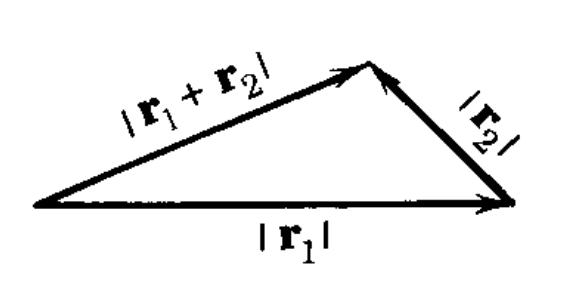
\includegraphics[width=0.9\linewidth]{figures/triangle vectors sum.png}
                \caption{}
                \label{fig:triangle vectors sum}
            \end{wrapfigure}

            \paragraph{$\bullet$} Note,  $f(\vec{r}) = |\vec{r}|$ is not a linear function, because the length 
            of the sum of two vectors is not in general the sum of their lengths. That is,
            $$ f(\vec{r_1} + \vec{r_2}) = |\vec{r_1} + \vec{r_2}| \neq |\vec{r_1}| + |\vec{r_2}| = 
            f(\vec{r_1}) + f(\vec{r_2})$$ as in Fig.\eqref{fig:triangle vectors sum}.
            Also noticw that we call $y=ms+b$ a linear a equation, however the function
            $f(x)=mx+b$ is not linear by the test \eqref{eq:A function of a vector} 
            (unless $b=0$).

            \paragraph{$\bullet$} Now consider \textbf{vector function} of a vector $\vec{r}$
            \coloredeq{eq:vector function}
            {
                \begin{aligned}
                    \text{$\vec{F}(\vec{r})$ is a linear vector function if}&
                    \\
                    \vec{F}(\vec{r_1}+\vec{r_2}) &= \vec{F}(\vec{r_1}) + \vec{F}(\vec{r_2})
                    \quad and \quad
                    \vec{F}(a\vec{r}) = a\vec{F}(\vec{r})
                    \\
                    \text{where $a$ is a scalar.}
                \end{aligned}
            }

            \paragraph{$\bullet$} Recall that from calculus:
            \begin{align}
                \label{eq:differentiation of sum}
                \begin{aligned}
                    \frac{d}{dx}\left[ f(x) + g(x) \right] &= \frac{d}{dx}f(x) + \frac{d}{dx}g(x) \quad and\\
                    \frac{s}{dx}\left[ kf(x) \right] &= k\frac{d}{dx}f(x)\\
                    \text{where $k$ is a constant}
                \end{aligned}
            \end{align}

            This is silimilar to \eqref{eq:A function of a vector}, then we call $d/dx$ a \textbf{linear opreator}.
            An \textbf{operator} or \textbf{operation} simply means a rule or some kind of instruction telling us what 
            to do with whatever follows it. In other words, a \textit{linear operator} is a \textit{linear function}, so 
            
            \coloredeq{eq:A linear operator}{
                \begin{aligned}
                    \text{$O$ is a linear operator if}& \\
                    O(A+B) &= O(A) + O(B) \qquad and \qquad O(kA) = kO(A)\\
                    \text{where $k$ is a number}
                \end{aligned}
            }

            \paragraph{Matrix Operators, Linear Transformations} % (fold)
            \label{par:Matrix Operators, Linear Transformations}
            Consider the following equation set 
            \begin{align}
                \label{eq:transformation:1}
                \begin{cases}
                    X = ax + by \\
                    Y = cx + dy
                \end{cases}
                \qquad or \qquad 
                \begin{bmatrix}
                    X \\ Y
                \end{bmatrix} = 
                \begin{bmatrix}
                    a & b \\
                    c & d
                \end{bmatrix}
                \begin{bmatrix}
                    x \\ y
                \end{bmatrix}
                \qquad or \qquad 
                R = Mr
            \end{align}
            where $a$, $b$, $c$, and $d$ are constants.
            For every point $(x,y)$, these equations results a point $(X, Y)$.

            If we think of each point of the $(x, y)$ plane being moved to some other 
            point (the origin not being moved), we can call this 
            process a \textbf{mapping} or \textbf{transformation} of the plane into itself. All the information 
            about this \textit{transformation} is contained in the matrix $M$. We say that this matrix is 
            an \textit{operator} which maps the plane into itself.
            
            \begin{wrapfigure}{r}{0.2\linewidth}
                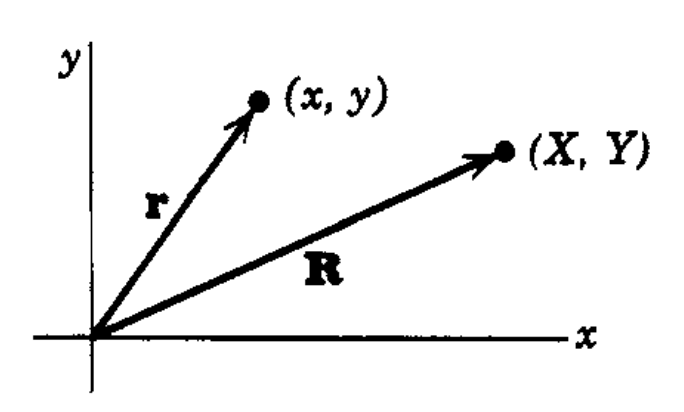
\includegraphics[width=0.9\linewidth]{figures/transformation1.png}
                \caption{fixed coordinates axes}
                \label{fig:transformation1}
                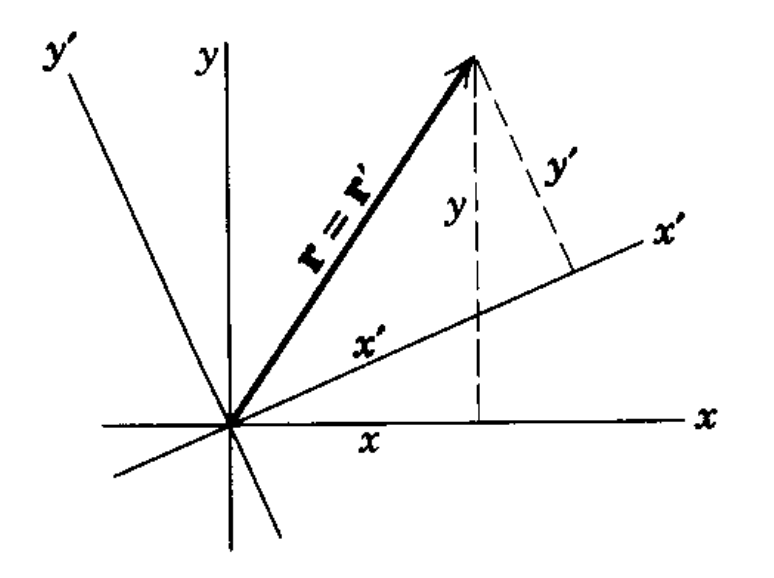
\includegraphics[width=0.9\linewidth]{figures/transformation2.png}
                \caption{A fixed vector}
                \label{fig:transformation2}
            \end{wrapfigure}

            \paragraph{$\bullet$}Any matrix can be thought of as an \textit{operator} 
            on (conformable) column matrices $r$. From \eqref{eq:A linear operator}, $M$ is a linear operator.
            
            \paragraph{$\bullet$}We can interpreted Eqs.\eqref{eq:transformation:1} geometrically in two ways. In Fig.\eqref{fig:transformation1}
            The vector $\vec{r}$ has been changed to the vector $\vec{R}$ by the transformation \eqref{eq:transformation:1}.
            
            \paragraph{$\bullet$}However, in Fis.\eqref{fig:transformation2} \texttt{two} sets of coordinates 
            axes $(x, y)$ and $(x', y')$, and \texttt{one} vector $\vec{r} = \vec{r^\prime}$. The
            transformation can ve written as 
            \begin{align}
                \label{eq:transformation:2}
                \begin{cases}
                    x' = ax + by \\
                    y' = cx + dy
                \end{cases}
                \qquad or \qquad 
                \begin{bmatrix}
                    z'\\ y'
                \end{bmatrix} = 
                \begin{bmatrix}
                    a & b \\
                    c & d
                \end{bmatrix}
                \begin{bmatrix}
                    x \\ y
                \end{bmatrix}
                \qquad or \qquad 
                r' = Mr
            \end{align}
            % paragraph Matrix Operators, Linear Transformations (end)

            \paragraph{Orthogonal Transformations} % (fold)
            \label{par:Orthogonal Transformations}
            This is a special case of a \textit{linear transformation} which preserves the length of a vector.
            In \eqref{eq:transformation:2} is an \textit{orthogonal transformation} if
            \begin{align}
                \label{eq:orthogonal condition}
                x'^2 + y'^2  = x^2 + y^2
            \end{align}
            then either it is reflected or rotated. The matrix \textit{M} of an orthogonal transformation is called an \textbf{orthogonal matrix}.
            The inverse of an orthogonal matrix equals its transpose. \coloredeq{eq:orthogonal matrix}{M^{-1} = M^T, \quad M \text{ is orthogonal}}
            From Eq.\eqref{eq:transformation:2} and \eqref{eq:orthogonal condition}
            \begin{align*}
                x'^2 + y'^2 &= (ax + by)^2 + (cx + dy)^2 \\
                            &=(a^2 +c^2)x^2 +2(ab+cd)xy+(b^2 +d^2)y^2 \equiv x^2 +y^2\\
                        \end{align*}
            Thus we must have $a^2 +c^2=b^2 +d^2=1,\quad ab+cd=0$
            \begin{align*}
                \begin{aligned}
                    MM^T &= \begin{bmatrix}
                        a & c \\ b & d
                    \end{bmatrix}
                    \begin{bmatrix}
                        a & b \\ c & d
                    \end{bmatrix} = 
                    \begin{bmatrix}
                        a^2 +c^2 & ab+cd \\
                        ab+cd & b^2 +d^2
                    \end{bmatrix}
                    \equiv \begin{bmatrix}
                        1 & 0 \\ 0 & 1
                    \end{bmatrix}
                \end{aligned}
            \end{align*}
                                
            Let Eq.\eqref{eq:orthogonal matrix} be $MM^T=I$ and from Eq.\eqref{eq:multiplication of determinants} we have
            \begin{align*}
                \det{M^TM} &= \det{M^T} \det{M}\\
                and \quad det{M^T} &= \det{M}\\
                so\quad \det{M}^2 &= \det{M^TM} = \det{I} = 1
            \end{align*}
            \coloredeq{eq:identity of orthogonal}{\det{M} = \pm 1}

            \paragraph{$\bigstar$} $\det{M} = 1$ corresponds geometrically to a \textit{rotation}, 
            and $\det{M} = -1$ means that a \textit{reflection} is involved.
            % paragraph Orthogonal Transformations (end)

            \begin{wrapfigure}{r}{0.2\linewidth}
                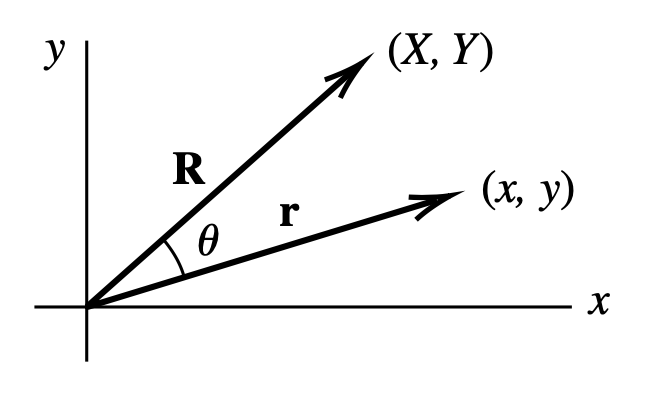
\includegraphics[width=0.9\linewidth]{figures/vectors rotation.png}
                \caption{Vectors rotation with an angle $\theta$}
                \label{fig:vectors rotation}
                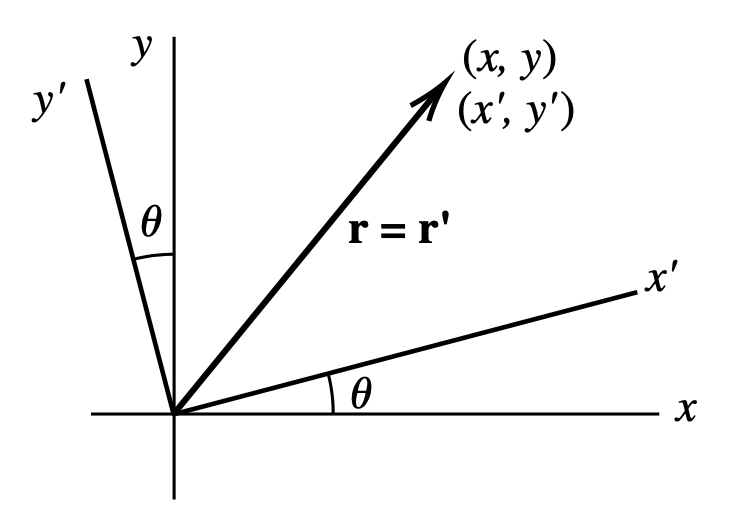
\includegraphics[width=0.9\linewidth]{figures/axes rotation.png}
                \caption{Axes rotation}
                \label{fig:axes rotation}
            \end{wrapfigure}

            \paragraph{Rotations in 2 Dimensions} % (fold)
            \label{par:Rotations in 2 Dimensions}
            In Fig.\eqref{fig:vectors rotation} we have two vectors $\vec{R}$  and $\vec{r}$ which is rotated by $\theta$.
            we can write in matrix their transformation as 
            \begin{align}
                \label{eq:vector rotation matrix}
                \begin{bmatrix}
                    X \\ Y
                \end{bmatrix} = 
                \begin{bmatrix}
                    \cos{\theta} & -\sin{\theta} \\
                    \sin{\theta} & \cos{\theta}
                \end{bmatrix} 
                \begin{bmatrix}
                    x \\ y
                \end{bmatrix}
            \end{align}
            
            \paragraph{$\bullet$} However for axes rotation as in Fig.\eqref{fig:axes rotation} we have 
            \begin{align}
                \label{eq:axes rotation matrix}
                \begin{bmatrix}
                    x' \\ y'
                \end{bmatrix} = 
                \begin{bmatrix}
                    \cos{\theta} & \sin{\theta} \\
                    -\sin{\theta} & \cos{\theta}
                \end{bmatrix} 
                \begin{bmatrix}
                    x \\ y
                \end{bmatrix}
            \end{align}

            \paragraph{$\bullet$} Both Eq.\eqref{eq:vector rotation matrix} and Eq.\eqref{eq:axes rotation matrix} are called \textbf{rotation equations}
            and the matrices that contain $\theta$ are called \textbf{rotation matrices}. Also notice that Eq.\eqref{eq:vector rotation matrix} 
            and Eq.\eqref{eq:axes rotation matrix} are inverses of each other.
            % paragraph Rotations in 2 Dimensions (end)

            \paragraph{Rotations and Reflections in 3 Dimensions} % (fold)
            \label{par:Rotations and Reflections in 3 Dimensions}
            For a vector $ \vec{r} = \langle x, y, z \rangle$. The the following matrix is a rotation about $z-axis$,
            \begin{align}
                \label{eq:rotation about z}
                \begin{bmatrix}
                    \cos{\theta} & -\sin{\theta} & 0 \\
                    \sin{\theta} & \cos{\theta} & 0 \\
                    0 & 0 & 1
                \end{bmatrix}
            \end{align}
            And the following is a rotation and reflection about $xy-plane$
            \begin{align}
                \label{eq:rotationa z and reflection in xy}
                \begin{bmatrix}
                    \cos{\theta} & -\sin{\theta} & 0 \\
                    \sin{\theta} & \cos{\theta} & 0 \\
                    0 & 0 & -1
                \end{bmatrix}
            \end{align}
            % paragraph Rotations and Reflections in 3 Dimensions (end)

        
            
        \section{Linear Dependence and Independence}

            In general, a set of vectors is linearly dependent, if  there are some linear combinations of them equals \textit{zero} (other than all the coefficients 
            equal zero). We can use row reduction to form linear combinations by \textit{elementary row operations}. These operations are reversible, se we can combine
            the remaining vectors to form the original vectors. Thus the remaining vectors are \textit{independent} and called as \textit{basis vectors}.

            \paragraph{Linear Independence of Functions} % (fold)
            \label{par:Linear Independence of Functions}
            Similar to vectors, the functiond $f_1(x),\, f_2(x),\, \dots , f_n(x)$ are linearly dependent if there are some linear combinations of them is identically
            \textit{zero}, meaning, if there are constants $k_1, k_2, \dots , k_n$ (not all zero), such that,
            \begin{align*}
                k_1 f_1(x) + k_2 f_2(x) + \dots +k_n f_n(x) \equiv 0
            \end{align*}

            For a given set of functiond we have the fillowing theorem
            \coloredeq{eq:set of functions dependence}{
                \begin{aligned}
                    \text{if $f_1(x),\, f_2(x),\, \dots , f_n(x)$ have derivatives of order $n-1$ and if the determinant} & \\
                    W = \begin{vmatrix}
                        f_1(x) & f_2(x) & \dots & f_n(x) \\
                        f'_1(x) & f'_2(x) & \dots & f'_n(x) \\
                        f''_1(x) & f''_2(x) & \dots & f''_n(x) \\
                        \vdots & \vdots & \ddots & \vdots \\
                        f_1^{n-1}(x) & f_2^{n-1}(x) & \dots & f_n^{n-1}(x) \\
                    \end{vmatrix} \neq 0 & \\
                    \parbox{0.85\linewidth}{then the functions are linearly independent. the determinant of $W$ is called \textit{Wronskian} of the functions.
                    If $W \equiv 0$, it is not necessarily imply "functions dependent".}
                \end{aligned}
            }
            % paragraph Linear Independence of Function (end)

            \paragraph{Homogeneous Equations} % (fold)
            \label{par:Homogeneous Equations}
            We consider a set of equations, but a special case raises when the all the right side of those equations are zero.
            
            \coloredeq{homogeneous equations:1}{\parbox[t][3\baselineskip][c]{0.9\linewidth}{
                Homogeneous equations are never \textit{inconsistent}; they always have the solution "all unkowns $=0$" (called \textit{trivial solution}). If the number of 
                the independent \textit{equations} (the rank of the matrix) is the same as the the number of the \textit{unknowns}, this is the only solution. If the 
                \textit{rank} is less than the \textit{unknowns}, there are infinitely many solutions.
            }}

            \bulletpar For $n$ homogeneous equations in $n$ unknowns, they have only a trivial solution, unless their rank is less than $n$. Meaning that, at least one row
            of the reduced $n$ by $n$ coefficients matrix is zero row. Then its determinant is zero. Thus we say
            \coloredeq{homogeneous equations:2}{\parbox[t][2\baselineskip][c]{0.9\linewidth}{
                A system of $n$ homogeneous equations in $n$ unknowns has solutions other than the trivial solution iff the determinant of the coefficients is zero
            }}
            % paragraph Homogeneous Equations (end)

        \section{Special Matrices and Formulas}
            There are some importants special matrices. Consider a matrix $A$, so

            \begin{center}
                \begin{tabular}{m{11em} m{10em} m{10em}}
                    \hline
                    Name of matrix & Notations & Procedure \\
                    \hline\hline
                    Transponse of $A$. & $A^T$ or \~A or $A'$ & Interchange rows and columns in $A$. \\

                    Complex conjugate of $A$. & $\bar{A}$ or $A^*$ & The complex conjugate of each element in $A$. \\

                    Transponse conjugate,\newline Hermitian conjugate,\newline adjoint,\newline Hermitian adjoint.\newline & 
                    $A^\dagger$ & The complex conjugate of each element in $A^T$.\\

                    Inverse of $A$ & $A^{-1}$ & See Par.\eqref{par:Inverse of a Matrix}\\

                \end{tabular}
                \label{tab:special matrices}
            \end{center}
            Also the following are special properties, 
            \begin{center}
                \begin{tabular}{l l}
                    \hline
                    A matrix is & if it satisfies\\
                    \hline \\
                    real           & $A = \bar{A}$ \\
                    symmetric      & $A = A^T$, $A$ real \\
                    skew-symmetric or antisymmetric & $A = -A^T$, $A$ real \\
                    orthogonal     & $A^{-1} = A^T$, $A$ real \\
                    pure imaginary & $A = - \bar{A}$ \\ 
                    Hermitian      & $A = A^\dagger$ \\
                    anti-Hermitian & $A = - A^\dagger$ \\
                    unitary        & $A^{-1} = A^\dagger$ \\
                    normal         & $A A^\dagger = A^\dagger A$\\
                    \hline
                \end{tabular}
                \label{tab:matrix special properties}
            \end{center}

            \paragraph{Kronecker $\sigma$} is defined  as 
            \coloredeq{eq:Kronecker}{
                \sigma_{ij} = \begin{cases}
                    1, &\text{ if }i=j\\
                    0, &\text{ if }i \neq j
                \end{cases}
            }
            We can define the unit matrix as one whose elements $I = \sigma_{ij}$. We use Eq.\eqref{eq:matrix multiplication in indeces} to prove
            matrix associative law for matrix, that is 
            $$ A(BC) = (AB)C = ABC $$
            First we write, $(BC)_{kj} = \sum_l B_{kl} C_{li}$ then we have
            \begin{align*}
                [A(BC)]_{ij} &= \sum_k A_{ik} (BC)_{kj} = \sum_k A_{ik}\, \sum_l B_{kl} C_{lj} \\
                             &= \sum_k \sum_l A_{ik} B_{kl} C_{lj} = (ABC)_{ij}
            \end{align*}
            which is the index notation of $A(BC)= ABC$.

            Silimilarly, we can fins the transpose of the product ot two matrices. Recall that $A_{ik}^T = A_{ki}$.
            \begin{align*}
                (AB)_{ik}^T &= (AB)_{ki} = \sum_j A_{kj} B_{ji} = \sum_j A_{jk}^T B_{ij}^T \\
                            &=\sum_j B_{ij}^T A_{jk}^T = (B^T A^T)_{ik} \\
                    (AB)^T &= B^T A^T
            \end{align*}
            In general, 
            \coloredeq{eq:associative trnsponse}{
                \begin{aligned}
                    \parbox[t]{0.6\linewidth}{The transpose of a product of matrices is equal to the product of the transposes in \underline{reverse order}.}
                \end{aligned} &&
                (ABCD)^T = D^T D^T B^T A^T
            }
            A similar theorem foe the inverse
            \coloredeq{eq:associative inverse}{
                \begin{aligned}
                    \parbox[t]{0.5\linewidth}{The inverse of a product of matrices is equal to the product of the inverses in \underline{reverse order}.}
                \end{aligned} &&
                (ABCD)^{-1} = D^{-1} D^{-1} B^{-1} A^{-1}
            }

            \paragraph{Trace of a Matrix} % (fold)
            \label{par:Trace of a Matrix}
            The \textbf{trace} (or \textbf{spur}) of a matrix $A$ is the sum of the elements in the main diagonal.\\
            \fbox{The trace of a product of matrices is not changed by arrange them in cyclic order}. Meaning that,
            \begin{align*}
                \tr{ABC} = \tr{BCA} = \tr{CAB}
            \end{align*}
            proof,
            \begin{align*}
                \tr{ABC} = \sum_i (ABC)_{ii} &= \sum_i \sum_j \sum_k A_{ij} B_{jk} C_{ki} \\
                                            &= \sum_i \sum_j \sum_k B_{jk} C_{ki} A_{ij} = \tr{BCA} \\
                                            &= \sum_i \sum_j \sum_k C_{ki} A_{ij} B_{jk} = \tr{CAB}
            \end{align*}
            \textit{Heads up}: In general $\tr{ABC}$ is not equal to $\tr{ACB}$. To memorize it, take the last matrix an insetrt it before the first one, and on.
            % paragraph Trace of a Matrix (end)
        \section{Linear Vector Spaces}
            We dealt with vectors such that $\vec{r} = x\ihat + y\jhat + z\khat$, that represents a vector from the origin to the point $(x, y, z)$. The all possible 
            sets of vectors make up a 3-dimensional space $R_3$ ($R$ for real) or $V_3$ ($V$ for vector) or $E_3$ ($E$ for Euclidean). Generally, an ordered set of $n$
            points or vectors make up a $n$-dimensional space $V_n$. All the termonolgy are also aplies for $n$-D, such the distance and the orthogonality.
            
            \paragraph{Subspace, Span, Basis, Dimension} % (fold)
            \label{par:Subspace, Span, Basis, Dimension}

            \bulletpar Two vectors in 3-dimensional space represent a plane, or a vector space $V_2$. All thier possible combinations lie on that plane. Thye are also a 
            a part of $V_3$, we say that $V_2$ is a \textit{subspace} of $V_3$.

            \bulletpar A set of vectors \textbf{spans} a space if all the vectors in the space be written as linear combinations of the spanning set. A \textit{basis} vector is 
            a set of \textit{linearly independent} vectors which span a vector space. 

            \bulletpar A \textit{dimension} of a vector space is equal to the number of the basis vectors. \\
            For example, the three unit vectors $\ihat, \jhat, \khat$ span the vector space $V_3$; they are linearly independent, thus a basis for the space $V_3$.
            % paragraph Subspace, Span, Basis, Dimension (end)

            \paragraph{Inner Product, Norm, Orthogonality} % (fold)
            \label{par:Inner Product, Norm, Orthogonality}
            Let us generalize the the dot product in Eq\eqref{eq:dot product} to $n$ dimensions
            \coloredeq{eq:dot product to nD}{\vec{A} \cdot \vec{B} = \sum_{i=1}^n A_i B_i}

            Similarly, to generalize the \textit{norm} of $\vec{A}$
            \coloredeq{eq:norm to nD}{A = |\vec{A}| = \sqrt{\vec{A} \cdot \vec{A}} = \sqrt{\sum_{i=1}^n A^2_i}}
            For orthogonality we have 
            \coloredeq{eq:orthogonality to nD}{\text{$\vec{A}$ and $\vec{B}$ are orthogonal if}\qquad  \sum_{i=0}^n A_i B_i=0}
            % paragraph Inner Product, Norm, Orthogonality (end)

            \paragraph{Schwarz Inequality} % (fold)
            \label{par:Schwarz Inequality}
            We can also use the formula $\vec{A} \cdot \vec{B} = AB \cos{\theta}$ to find the angle between two vectors in $n$-dimensions. The result must satisfy
            $|\cos{\theta}| \leq 1$, thus 
            \coloredeq{eq:Schwarz inequality}{|\vec{A} \cdot \vec{B}| \leq AB, \qquad or \quad 
            \left|\sum_{i=1}^n A_i B_i \right| \leq \sqrt{\sum_{i=1}^n A^2_i} \sqrt{\sum_{i=1}^n B^2_i}}
            \textit{Proof}: if $\vec{B} = \vec{0}$, Eq.\eqref{eq:Schwarz inequality} is stisfied. If $\vec{B} \neq \vec{0}$, consider the vector 
            $\vec{C} = B\vec{A} - (\vec{A} \cdot \vec{B})\vec{B}/B$. Then, $\vec{C} \cdot \vec{C} = \sum C_i^2 \geq 0 $
            \begin{align*}
                \vec{C} \cdot \vec{C} &= B^2 (\vec{A} \cdot \vec{A}) - 2B(\vec{A} \cdot \vec{B})(\vec{A} \cdot \vec{B})/B + (\vec{A} \cdot \vec{B})^2 
                (\vec{B} \cdot \vec{B})/B^2 \\
                &= A^2 B^2 -2(\vec{A} \cdot \vec{B})^2 + (\vec{A} \cdot \vec{B})^2 \\
                &= A^2 B^2 - (\vec{A} \cdot \vec{B})^2 = C^2 \geq 0
            \end{align*}
            Thus we can define the angle between two vectors as $\cos{\theta} = \vec{A} \cdot \vec{B} / AB$.
            % paragraph Schwarz Inequality (end)

            \paragraph{Orthonormal Basis; Gram-Schmidt Method} % (fold)
            \label{par:Orthonormal Basis; Gram-Schmidt Method}
            We call a set of vectors \textbf{orthonormal} if they are all mutually \textit{orthogonal} (perpendicular), and each vector is \textit{normal}ized;
            $\ihat$, $\jhat$, and $\khat$ as an example. 
            
            \bulletpar Consider we have three basis vectors $\vec{A}$, $\vec{B}$, and $\vec{C}$. First, normalize $\vec{A}$. Substract 
            from $\vec{B}$ its projection along $\vec{A}$, then normalize it. And so on.
            % paragraph Orthonormal Basis; Gram-Schmidt Method (end)

            \paragraph{Complex Euclidean Space} % (fold)
            \label{par:Complex Euclidean Space}
            It is allowed to have a vector with components of comlex numbers. In Eq.\eqref{eq:dot product to nD} we need to make what under the square root positive. So 
            we replace $A^2_i$ by $|A_i|^2 = A^*_i A_i$. likewise, in Eq.\eqref{eq:norm to nD}, Eq.\eqref{eq:orthogonality to nD}, and Eq.\eqref{eq:Schwarz inequality}.
            \begin{align*}
                \vec{A} \cdot \vec{B} = \sum_{i=1}^n A^*_i B_i \\
                |\vec{A}| = \sqrt{\sum_{i=1}^n A^*_i A_i}
            \end{align*}
            \bulletpar In matrix form, suppose that $A$ is a column matrix with elemnts $A_i$. Then its transpose conjugate $A^\dagger$ is a row matrix with elements 
            $A^*_i$. We can write, $\sum A^*_i B_i = A^\dagger B$.
            % paragraph Complex Euclidean Space (end)

        \section{Eigenvalues and Eigenvectors; Diagonalizing Matrices}
            In some special matrix transformation, there are some specific vectors that do not move off of their span; such vectors are called 
            \textbf{eigenvectors}. They satisfiy $\vec{R} = \lambda \vec{r}$, where $\lambda$ is called the \textbf{eigenvalue}.

            \bulletpar \textbf{Eigenvalues} Consider the transformation of $\vec{R} = M\vec{r}$,
            \begin{align}
                \label{eq:eigenvalue:1}
                \begin{bmatrix}
                    X \\ Y
                \end{bmatrix} = 
                \begin{bmatrix}
                    a & b \\ c & d
                \end{bmatrix}
                \begin{bmatrix}
                    x \\ y
                \end{bmatrix}
            \end{align}
            The eigenvector condition $\vec{R} = \lambda \vec{r}$
            \begin{align}
                \label{eq:eigenvalue:2}
                \begin{bmatrix}
                    X \\ Y
                \end{bmatrix} = 
                \begin{bmatrix}
                    a & b \\ c & d
                \end{bmatrix}
                \begin{bmatrix}
                    x \\ y
                \end{bmatrix} = 
                \lambda \begin{bmatrix}
                    x \\ y
                \end{bmatrix}
            \end{align}
            Thus we get
            \begin{align}
                \label{eq:eigenvalue:3}
                \begin{bmatrix}
                    a - \lambda & b \\ c & d - \lambda
                \end{bmatrix} = 0 \qquad or
                \begin{cases}
                    (a- \lambda)x + b y = 0 \\
                    c x + (d- \lambda)y = 0
                \end{cases}
            \end{align}
            These are homogeneous equations. Thus from \eqref{homogeneous equations:1}, a set of homogeneous equations has a solution other than $x=y=0$, iff the 
            determinant of coefficients is zero.

            \coloredeq{finding the characteristic equation}{
                \text{For the maatrix } M = \begin{bmatrix}
                    a & b \\ c & d
                \end{bmatrix} &&
                \text{the characteristic equation is} \begin{vmatrix}
                    a - \lambda & b \\ c & d - \lambda
                \end{vmatrix} = 0
            }
            \bulletpar \textbf{Eigenvectors} By finding the the eigenvalue, $\lambda$, and substituting it back into Eq.\eqref{eq:eigenvalue:3}, will result line
            equations. Any vector from the origin to a point along those lines is considered as an eigenvector, where they stay in thier span.

            \paragraph{Diagonalizing a Matrix} % (fold)
            \label{par:Diagonalizing a Matrix}
            Again substitute the eigenvalues into Eq.\eqref{eq:eigenvalue:3}, and distinguish the eigenvectors by subscripts, 
            \begin{align}
                \label{eq:diagonalizing a matrix:1}
                \begin{aligned}
                    a x_1 + b y_1 = \lambda_1 x_1 && a x_2 + b y_2 = \lambda_2 x_2 \\
                    c x_1 + d y_1 = \lambda_1 x_1 && c x_2 + d y_2 = \lambda_2 x_2
                \end{aligned}
            \end{align}
            then by writing these equation as one matrix equation, \fbox{$MC = CD$}
            \begin{align}
                \label{eq:diagonalizing a matrix:2}
                \begin{bmatrix}
                    a & b \\ c & d
                \end{bmatrix} \begin{bmatrix}
                    x_1 & x_2 \\
                    y_1 & y_2
                \end{bmatrix} = \begin{bmatrix}
                    x_1 & x_2 \\
                    y_1 & y_2
                \end{bmatrix} \begin{bmatrix}
                    \lambda_1 & 0  \\ 0 & \lambda_2
                \end{bmatrix}
            \end{align}
            where $(x_1, y_1)$ is a point along the found line obtained from $\lambda_1$; which is the eigenvector of the transformation. If $\det{C} \neq 0$, then $C$ 
            has an inverse $C^{-1}$, so 
            \coloredeq{eq:diagonal matrix}{
                \parbox[t]{0.65\linewidth}{The matrix $D$ has nonzero numbers only in its main diagonal, so it is called \textbf{diagonal matrix}.
                Also, the matrix $D$ is called \textbf{similar} to $M$. When we obtain $D$ given $M$, we \textit{diagonalized} $M$ by a 
                \textit{similarity tranformation}} &&
                C^{-1}MC = D
            }
            \bulletpar The diagonalization process simplify problems by a better choice of variables. For example, it is simpler to to describe some of deformations by 
            using axes along the eigenvectors. Thus geometrically, 
            \bulletpar A complete example, consider two coordinate systems, $(x, y)$ and $(x', y')$, and two vectors that are beign transform from $\vec{r}=(x, y)$ into
            $\vec{R}=(X, Y)$. The $\vec{r}$ and $\vec{r'}$ in the two systems are related to each other by Eq.\eqref{eq:axes rotation matrix}, to find $(z, y)$,
            \begin{align}
                \begin{aligned}
                    \label{eq:diagonalization example:1}
                    x = x' \cos{\theta} - y' \sin{\theta} \\
                    y = x' \sin{\theta} + y' \cos{\theta}
                \end{aligned} \qquad \Leftrightarrow \quad 
                \begin{aligned}
                    r = C r', && C = \begin{bmatrix}
                        \cos{\theta} & -\sin{\theta} \\ \sin{\theta} & \cos{\theta}
                    \end{bmatrix}
                \end{aligned}
            \end{align}
            Similarly we have, $R = C R'$. Consider a transformation matrix $M$ in $(x, y)$ system, as
            \begin{align}
                \label{eq:diagonalization example:2}
                R = M r
            \end{align}
            Now, we can get the transformation equation in $(x', y')$ system by substituting in Eq.\eqref{eq:diagonalization example:2}, so
            \begin{align}
                \label{eq:diagonalization example:3}
                R' = C^{-1} M C r' \Leftrightarrow R' = D r'
            \end{align}
            Thus we conclude that
            \coloredeq{diagonal matrix meainig}{
                \parbox[t]{0.8\linewidth}{$D = C^{-1}MC$ is the transformation matrix described in the $(x', y')$ system, where $M$ describes the tranformation in the
                $(x, y)$ system.}
            }
            \starpar If $C$ is chosen to make $D$ a diagonal matrix, then the new axes $(x', y')$ are along the eigenvectors of $M$.
            If the eigenvectors are perpendicular, then the new axess $(x', y')$ are a set of perpendicular axes rotated by $\theta$ from 
            axes $(x, y)$.
            
            \bulletpar However, if $C$ is not an orthogonal matrix, then the axes $(x', y')$ are not perpendicular and $|\vec{r}| \neq |\vec{r'}|$.
            
            \bulletpar Thus, if the unit eigenvectors in matrix $C$; are perpendicular, then $C$ is \textit{orthogonal}. This is only if the matrix $M$ is 
            \textit{symmetric}.
            % paragraph Diagonalizing a Matrix (end)

            \paragraph{Degeneracy} % (fold)
            \label{par:Degeneracy}
            means two (or more) independent eigenvectors correspond to the same eigenvalue.\\
            For a \textit{symmetric} matrix, we saw that the eigenvectors corresponding to different eigenvalues are \textit{orthogonal}.
            % paragraph Degeneracy (end)

            \paragraph{Diagonalizing Hermitian Matrices} % (fold)
            \label{par:Diagonalizing Hermitian Matrices}
            We saw how to diagonalize symmetric matrices by \textit{orthogonal similarity transformation}. Consider thid analogy
            \begin{center}
                \begin{tabular}{c | c}
                    \hline Real & Complex \\ \hline \\
                    Symmetric $S^T = S$     & Hermitian $H^\dagger = H$ \\
                    Orthogonal $O^T = O^{-1}$ & Unitary $U^\dagger = U^{-1}$ \\
                    \hline
                \end{tabular}
            \end{center}
            \starpar The eigenvalues of a Hermitian matrix are always \textit{real}. \\
            Consider $H$ to be a Hermitian matrix, and $\vec{r}$ the column matrix of a non-zero
            eigenvector of $H$ corresponding to the eigenvalue $\lambda$. Thus the eigenvector condition is 
            \begin{align*}
                Hr = \lambda r
            \end{align*}
            Taking the transpose conjugate ($\dagger$) of this this equation, we get
            \begin{align*}
                (Hr)^\dagger = r^\dagger H^\dagger = r^\dagger H \qquad
                \text{and} \quad \lambda r \Rightarrow \lambda^* r^\dagger
            \end{align*}
            For a Hermitian matrix we have $H^\dagger = H$, $\lambda$ is just a number. Hence, 
            \begin{align*}
                Hr = \lambda r \qquad \text{and} \qquad r^\dagger H = \lambda^* r^\dagger
            \end{align*}
            Then multiply the left by the row matrix $r^\dagger$, and the right by the column matrix $r$,
            \begin{align*}
                r^\dagger Hr = \lambda r^\dagger r \qquad \text{and} \qquad r^\dagger H r = \lambda^* r^\dagger r
            \end{align*}
            Substracting the two equations we get  $(\lambda - \lambda^*) r^\dagger r = 0$. But we assumed $r \neq 0$, so $\Lambda^* = \lambda$, hence the eigenvalue 
            $\lambda$ is always \textit{real}.

            \bulletpar For a Hermitian matrix, the eigenvectors corresponding to two different eigenvalues are \textit{orthogonal}. Consider  this,
            \begin{align*}
                H r_1 = \lambda_1 r_1 \qquad H r_2 = \lambda_2 r_2
            \end{align*}
            \begin{align*}
                r_1^\dagger H r_2 = \lambda_1 r_1^\dagger r_2 = \lambda_2 r_1^\dagger r_2 \qquad \text{or} \quad (\lambda_1 - \lambda_2) r_1^\dagger r_2 = 0
            \end{align*}
            If $\lambda_1 \neq \lambda_2$, then $r_1 \cdot r_2 = 0$, hence, they are \textit{orthogonal}.

            \starpar If a matrix $M$ has a real eigenvalues and can be diagonalize by a \textbf{unitary similarity transformation}, then $M$ is \textit{Hermitian}.
            We state \fbox{MU = UD}
            \begin{align*}
                U^{-1} M U &= D \\
                (U^{-1} M U)^\dagger &= U^{-1} M^\dagger U = D^\dagger = D \\
                \text{thus}\quad U^{-1} M U &= U^{-1} M^\dagger U
            \end{align*}
            We get, $M = M^\dagger$, hence, $M$ is Hermitian.
            
            \coloredeq{Hermitian theorem}{\parbox[t]{0.8\linewidth}{
                A matrix has real eigenvalues and can be diagonalize by a \textit{unitary similarity transformation} iff it is \textbf{Hermitian}.
            }}
            But a \underline{real} Hermitian matrix is a symmetric matrix, and \underline{real} unitary is a orthogonal matrix, 
            
            \coloredeq{Symmetric theorem}{\parbox[t]{0.8\linewidth}{
                A matrix has real eigenvalues and can be diagonalize by a \textit{orthogonality similarity transformation} iff it is \textbf{symmetric}.
            }}
            The normal matrices include, symmetric, Hermitian, orthogonal, and unitary matrices, thus
            
            \coloredeq{Normal theorem}{\parbox[t]{0.8\linewidth}{
                A matrix has real eigenvalues and can be diagonalize by a \textit{unitary similarity transformation} iff it is \textbf{normal}.
            }}
            % paragraph Diagonalizing Hermitian Matrices (end)

            \paragraph{Powers and Functions of Matrices}
            For the matrix $M$ raised to the power $n$, we can use the diagonalization,
            \begin{align*}
                M^n = C D^n C^{-1} \qquad \text{where} \qquad D = C^{-1} M C
            \end{align*}
        \section{An Introduction to Groups}
            Consider $\pm 1, \pm i$. No matter what the products and powers of them we compute, we never get numbers other than these foure. This  property of a set 
            of elements with a law of combinations is called \textbf{closure}. We are interested in groups of matrices, that is, in matrix representaions os of groups.

            \paragraph{A Group} % (fold)
            \label{par:A Group}
            is a set ${A, B, C, \dots}$ of elements --can be numbers, matrices, or operations-- togather with a law of combinations of two elements,  having four 
            conditions 
            \begin{enumerate}
                \item \textit{Closure}: The combination of any two elements is an element of the group.
                \item \textit{Associative}: The of combination satisfies the associative law; $(AB)C = A(BC)$.
                \item \textit{Unit element}: There is a unit element $I$ with the property that $AI = IA = A$ for every element of the group.
                \item \textit{Inverse}: Every element of the group has an inverse in the group; like, for $A$, there is an element $B$ such that $AB = BA I$.
            \end{enumerate}
            
            \bulletpar Thus, the set $\pm 1, \pm i$ is valid under these conditions. The \textbf{order of a finite group} is the number of elements in the group. If the elements 
            of a group of order $n$ are of the form $A, A^2, A^3, \dots, A^n =1$, it is called a \textbf{cyclic group}.

            \bulletpar Hence $\pm 1, \pm i$ is a cyclic group of order 4. A \textbf{subgroup} is a subset which is itself a group. The whole group or the unit element, 
            are called \textbf{trivial subgroup}, any other subgroup is called \textbf{proper subgroup}.Here $\pm 1, \pm i$, has the proper subgroup $\pm 1$.
            % paragraph A Group (end)

            \bulletpar A \textit{group multiplication} refers to the law of combination for  the group.

            \bulletpar Two gourps are called \textbf{isomorphic} if their multiplication tables are identical except for the names we attach to the elements.
            
            \bulletpar If evrey two group elements \textit{commute}, the group is called \textbf{Abelian}.

            \bulletpar Two group elements $A$ and $B$ are called \textbf{conjugate} elements, if there is a a group element $C$ such that $C^{-1}AC = B$. By making $C$
            be successively one \textit{group element} after another, we can find all the \textit{group conjugate} of $A$. This set is called a \textbf{class}.
            